\documentclass{article}

\title{Complex Variables Sections 5, 8 Homework}
\author{Adam Buskirk}

\usepackage{amssymb,amsmath,amsthm}
\usepackage{tikz}
\usepackage[margin=1in]{geometry}

\newtheorem{theorem}[subsection]{Theorem}
\newtheorem{conjecture}[subsection]{Conjecture}
\newtheorem{lemma}[subsection]{Lemma}
\theoremstyle{definition}
\newtheorem{definition}[subsection]{Definition}

\newcommand{\R}{\mathbb{R}}
\newcommand{\N}{\mathbb{N}}
\newcommand{\Q}{\mathbb{Q}}
\newcommand{\Z}{\mathbb{Z}}
\newcommand{\p}[1]{\left(#1\right)}
\newcommand{\set}[1]{\left\{#1\right\}}
% \newcommand{\p}[1]{\left(#1\right)}

\begin{document}
\maketitle

Section 5: \# 2a, 10.

Section 8: \# 1, 2.

\section{Problem 5.2.a}
Complex conjugation and adding imaginary numbers should not affect the real component of
the values; hence $\operatorname{Re}(\bar{z}-i)=2$ is equivalent to 
$\operatorname{Re}(z)=2$, as depicted in Figure \ref{5-2-a}.
\begin{figure}[h]
\centering
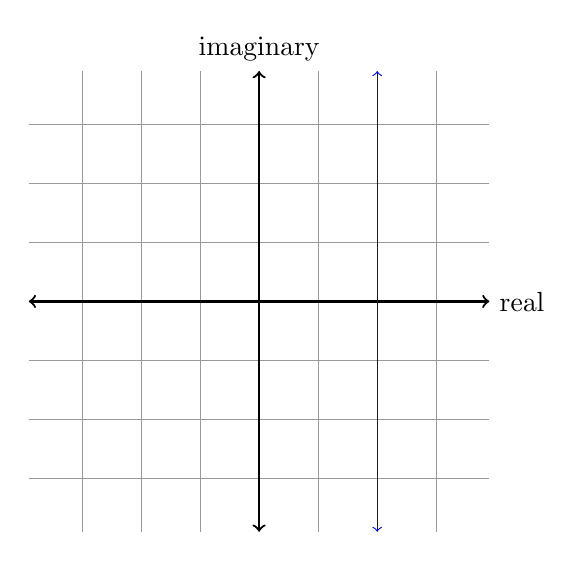
\begin{tikzpicture}[scale=0.75,domain=-4:4]
\draw[very thin,color=black!40] (-3.9,-3.9) grid (3.9,3.9);
\draw[thick,<->] (-3.9,0) -- (3.9,0) node[right] {real};
\draw[thick,<->] (0,-3.9) -- (0,3.9) node[above] {imaginary};
\draw[<->,color=blue] (2,-3.9) -- (2,3.9) ;
\end{tikzpicture}
\caption{The solutions to 5.2.a.}\label{5-2-a}
\end{figure}

\section{Problem 5.10}
\subsection{Part 5.10.a}
\begin{theorem}
$z$ is real if and only if $\bar{z}=z$.
\end{theorem}
\begin{proof}
If $z$ is real, $z=(x,0)$, so $z=(x,0)=(x,-0)=\bar{z}$.

If $z$ is not real, then $z=(x,y)$ for nonzero $y$. Then $z=(x,y)$ and $\bar{z}=(x,-y)$, 
which are not equivalent since $y \neq -y$.
\end{proof}
\subsection{Part 5.10.b}
\begin{theorem}
$z$ is either real or pure imaginary iff $\bar{z}^2=z^2$.
\end{theorem}
\begin{proof}
Suppose $z$ is either real or pure imaginary. Then, regardless, $z^2$ is real (obviously in the real
case; in the pure imaginary case, $z^2=(0,y)^2=(-y^2,0)$.). Since 
$z^2$ is real, $z^2 = \overline{z^2} = \bar{z}^2$.

If $\bar{z}^2 = \overline{z^2} = z^2$, this implies $z^2$ must be real. So if $z=(x,y)$, then 
$\operatorname{Im}(z^2) = \operatorname{Im}(x^2-y^2,2xy)=2xy=0$. Thus, either $x=0$ or $y=0$; 
in the former case, $z$ is purely imaginary, and in the latter $z$ is real. Thus $z$ is either
real or purely imaginary.
\end{proof}

\section{Problem 8.1}
\subsection{Part 8.1.a}
\begin{align*}
\arg(z)
&= \arg\p{\frac{i}{-2-2i}} \\
&= \arg(i) - \arg(-2-2i) \\
&= \pi/2 - (-3\pi/4) + 2\pi\Z \\
&= 2\pi/4 + 3\pi/4 + 2\pi\Z \\
&= 5\pi/4 + 2\pi\Z \\
&= -3\pi/4 + 2\pi\Z \\
\operatorname{Arg}(z) &= -3\pi/4
\end{align*}

\subsection{Part 8.1.b}
\begin{align*}
z
&= \arg\p{ \p{\sqrt{3}-i}^6 } \\
&= 6 \cdot \arg\p{\sqrt{3}-i} \\
&= 6 \cdot (-\pi/6 + 2\pi\Z)  \\
&= (-\pi/6)+(-\pi/6)+(-\pi/6) \\
&\qquad+(-\pi/6)+(-\pi/6)+(-\pi/6)+2\pi\Z \\
&= -\pi + 2\pi\Z \\
&= \pi + 2\pi\Z \\
\operatorname{Arg}(z) &= \pi 
\end{align*}
It is essential to note that the multiplication by 6 above is not the coset $6+2\pi\Z$ in the 
quotient field $\R/2\pi\Z$ which the $\arg$ generally occupies, but rather the action of 
the integer $6$ 
in that field on the coset-valued return of the $\arg$ above, as in a $\Z$-module. It does 
\textit{not} stretch the coset into $-\pi+12\pi\Z$.

\section{Problem 8.2}
\subsection{Problem 8.2.a}
\begin{theorem}
\[|e^{i\theta}|=1\]
\end{theorem}
\begin{proof}
Using the definitions of $e^{i\theta}$ and the modulus,
\begin{align*}
|e^{i\theta}| 
&= \left| \cos\theta+i\sin\theta \right| \\
&= \sqrt{(\cos\theta+i\sin\theta)(\cos\theta-i\sin\theta)}\\
&= \sqrt{ \cos^2\theta + \sin^2\theta }\\
&= \sqrt{1}\\
&= 1
\end{align*}
\end{proof}
\subsection{Problem 8.2.b}
\begin{theorem}
\[ \overline{e^{i\theta}} = e^{-i\theta} \]
\end{theorem}
\begin{proof}
\begin{align*}
\overline{e^{i\theta}} 
&= \overline(\cos\theta,\sin\theta) \\
&= (\cos\theta,-\sin\theta) \\
&= (\cos(-\theta),\sin(-\theta)) \\
&= e^{-i\theta}
\end{align*}
\end{proof}
\end{document}
